\documentclass[11pt]{article}
\usepackage[utf8]{inputenc}
\usepackage{geometry}
\geometry{a4paper, margin=1in}
\usepackage{graphicx}
\usepackage{amsmath}
\usepackage{booktabs}
\usepackage{multirow}
\usepackage{hyperref}
\usepackage{float}

\title{\textbf{Performance Analysis Naive Matrix Multiplication vs. Tiled Matrix Multiplication}}
\author{Joel Maldonado}
\date{\today}

\begin{document}

\maketitle

\section{Introduction}
This report compares two GPU matrix multiplication kernels:
a basic matrix multiplication implementation that accesses data directly from global memory,
and a tiled matrix multiplication implementation that uses shared memory to reuse data
within each thread block.

\section{Experimental Setup}
All experiments were executed in the same cluster. 
The hardware and software environment details are as follows:


\begin{itemize}
\item \textbf{GPU Model:} 1x NVIDIA Tesla P100 (16GB VRAM)
\item \textbf{Compute Capability:} 6.0
\item \textbf{CUDA Version:} 11.8
\item \textbf{Host CPU Allocation:} 1 Core
\item \textbf{Host RAM Allocation:} 6GB (6GB/core)
\end{itemize}

\section{Results \& Data}

\subsection{Execution Time Data}
The experiment ran both kernels on four test cases and
the configurations tests included thread block sizes of 4x4, 8x8, 16x16, and 32x32.
Each kernel was executed 10 times per configuration to obtain average execution times and standard deviations.
These results are summarized in Table \ref{tab:timing_data} below.
Additionally, note that for the tiled matrix multiplication algorithm,
we set the MAX\_TILE\_SIZE to 32 to accommodate the largest block size tested.
\begin{table}[H]
\centering
\renewcommand{\arraystretch}{1.3}
\begin{tabular}{|l|l|c|c|c|c|}
\hline
\multicolumn{6}{|c|}{\textbf{Execution Time Data (ms)}} \\
\hline
& & \multicolumn{4}{c|}{\textbf{Thread block configuration}} \\
\hline
& \textbf{Test case} & \textbf{4x4} & \textbf{8x8} & \textbf{16x16} & \textbf{32x32} \\
\hline
\multirow{4}{*}{\shortstack[l]{Basic Matrix\\Multiply}}
& Case 1 (2048x2048) & 120.1 $\pm$ 1.9 & 58.4 $\pm$ 1.3 & 45.3 $\pm$ 0.0 & 43.2 $\pm$ 0.1 \\ \cline{2-6}
& Case 2 (2051x2051) & 118.7 $\pm$ 1.7 & 58.5 $\pm$ 0.3 & 52.8 $\pm$ 0.1 & 56.1 $\pm$ 0.2 \\ \cline{2-6}
& Case 3 (4096x2048) & 481.8 $\pm$ 2.3 & 235.9 $\pm$ 2.6 & 183.0 $\pm$ 3.2 & 171.3 $\pm$ 2.9 \\ \cline{2-6}
& Case 4 (4096x2047) & 485.7 $\pm$ 2.7 & 242.9 $\pm$ 3.3 & 201.3 $\pm$ 3.5 & 214.5 $\pm$ 3.1 \\
\hline
\multirow{4}{*}{\shortstack[l]{Tiled Matrix\\Multiply}}
& Case 1 (2048x2048) & 251.0 $\pm$ 0.0 & 38.4 $\pm$ 0.0 & 14.2 $\pm$ 0.0 & 11.1 $\pm$ 0.6 \\ \cline{2-6}
& Case 2 (2051x2051) & 257.9 $\pm$ 3.4 & 38.2 $\pm$ 0.2 & 16.2 $\pm$ 0.1 & 12.1 $\pm$ 0.0 \\ \cline{2-6}
& Case 3 (4096x2048) & 954.3 $\pm$ 8.9 & 143.5 $\pm$ 2.9 & 59.3 $\pm$ 3.4 & 45.8 $\pm$ 0.0 \\ \cline{2-6}
& Case 4 (4096x2047) & 956.1 $\pm$ 6.8 & 144.6 $\pm$ 3.5 & 59.2 $\pm$ 2.8 & 45.8 $\pm$ 0.0 \\
\hline
\end{tabular}
\caption{Average kernel execution times over 10 iterations.}
\label{tab:timing_data}
\end{table}

\subsection{Speedup Analysis}

To better quantify the benefit of shared-memory tiling, we compute the
speedup of the tiled matrix multiplication algorithm relative to the basic matrix multiplication algorithm:
\[
\text{Speedup} = \frac{T_{\text{basic}}}{T_{\text{tiled}}}
\]
where $T_{\text{basic}}$ and $T_{\text{tiled}}$ are the execution times
of the basic matrix multiplication algorithm and the tiled matrix multiplication algorithm respectively.
Table~\ref{tab:speedup_data} shows the speedup using the best-performing
block configuration for both kernels.

\begin{table}[H]
\centering
\begin{tabular}{|c|c|}
\hline
\textbf{Test Case} & \textbf{Speedup (Basic Algorithm / Tiled Algorithm)} \\
\hline
Case 1 (2048$\times$2048) & 3.89$\times$ \\
Case 2 (2051$\times$2051) & 4.64$\times$ \\
Case 3 (4096$\times$2048) & 3.74$\times$ \\
Case 4 (4096$\times$2047) & 4.68$\times$ \\
\hline
\end{tabular}
\caption{Speedup of the tiled matrix multiplication algorithm over the basic matrix multiplication algorithm using the 32$\times$32 block configuration.}
\label{tab:speedup_data}
\end{table}

The tiled matrix multiplication algorithm achieves between approximately
3.7$\times$ and 4.7$\times$ speedup across the tested workloads.
This improvement comes from reducing redundant global memory accesses.
Each element loaded into shared memory is reused by multiple threads,
which significantly lowers global memory bandwidth pressure.

\subsection{Performance Visualizations}
In this section we analyze the performance of both kernels
 across the different test cases and block sizes.
Figures \ref{fig:basic_plot} analyzes the performance of the
basic matrix multiplication algorithm. In Figure \ref{fig:tiled_plot} we observe
speedup of the tiled matrix multiplication algorithm, and in Figure
 \ref{fig:comparison_plot} we compare the performance of both algorithms
 side by side on the largest test case, Case 4.

\begin{figure}[H]
	\centering
	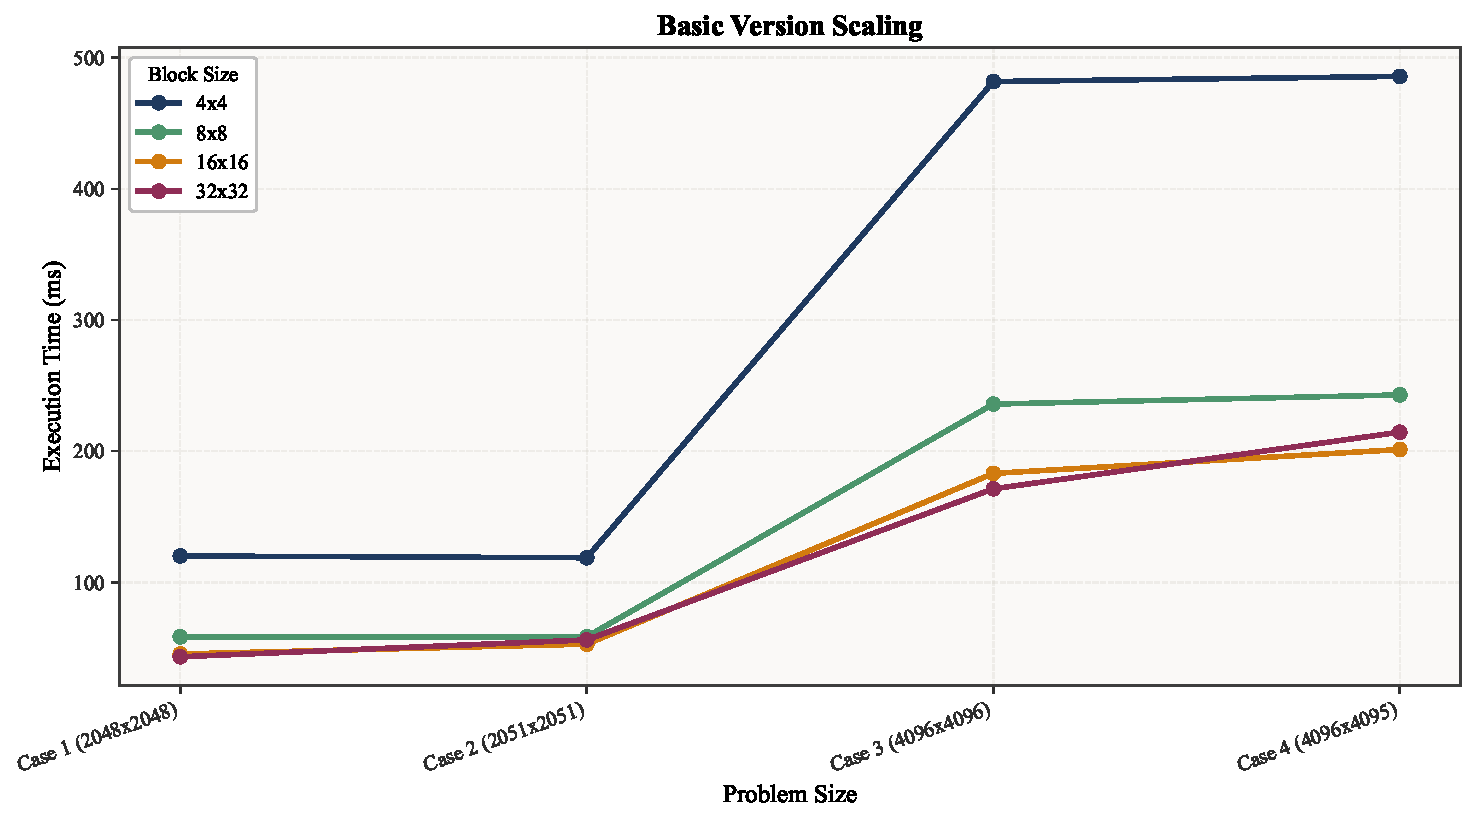
\includegraphics[width=0.9\textwidth]{../../ece569/build_dir/perf_analysis_graphs/plot1_basic_scaling.pdf}
	\caption{Execution time scaling for Basic Matrix Multiplication across block sizes.}
	\label{fig:basic_plot}
\end{figure}

\begin{figure}[H]
	\centering
	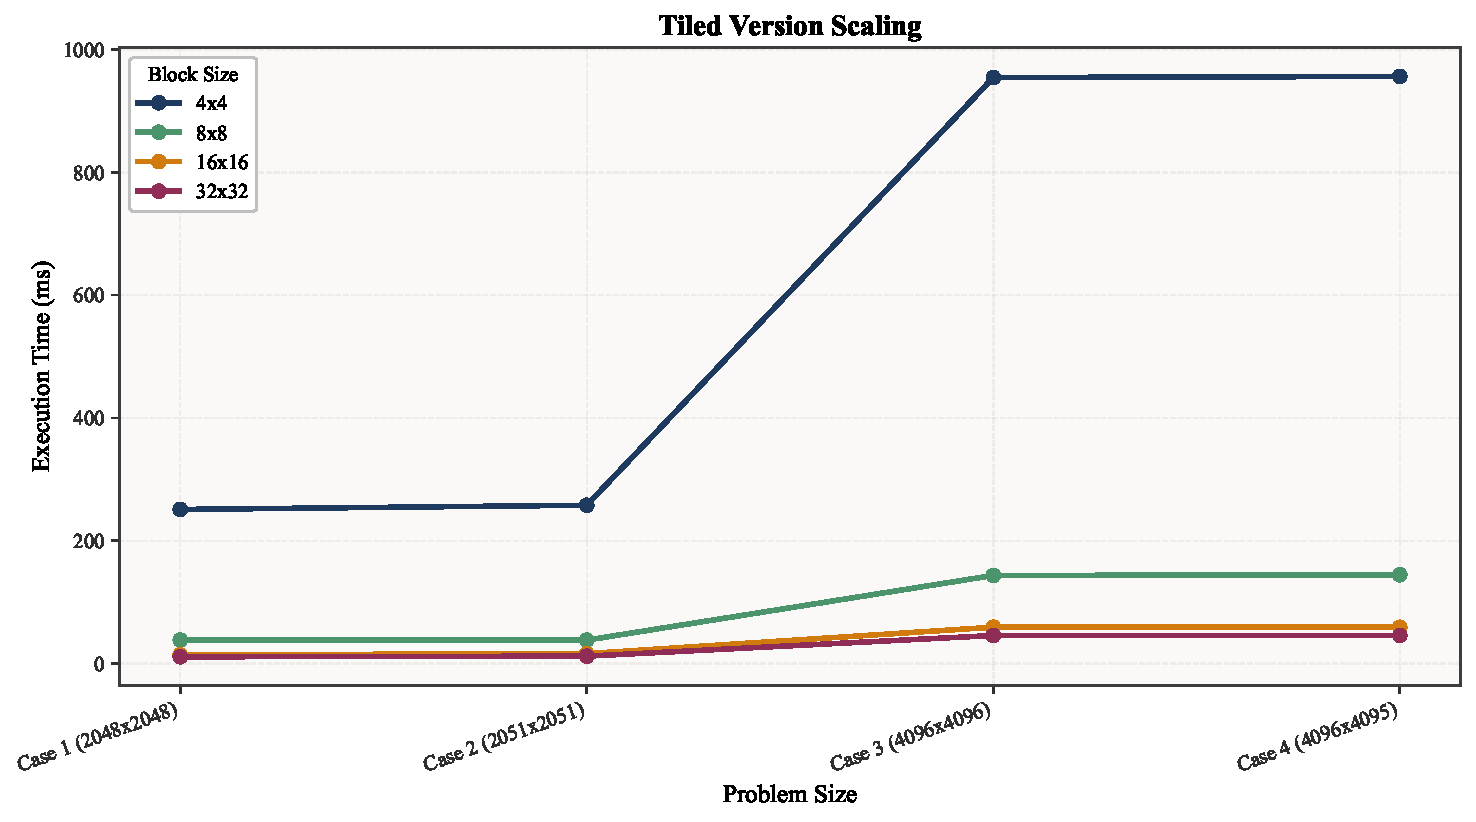
\includegraphics[width=0.9\textwidth]{../../ece569/build_dir/perf_analysis_graphs/plot2_tiled_scaling.pdf}
	\caption{Execution time scaling for Tiled Matrix Multiplication across block sizes.}
	\label{fig:tiled_plot}
\end{figure}

\begin{figure}[H]
	\centering
	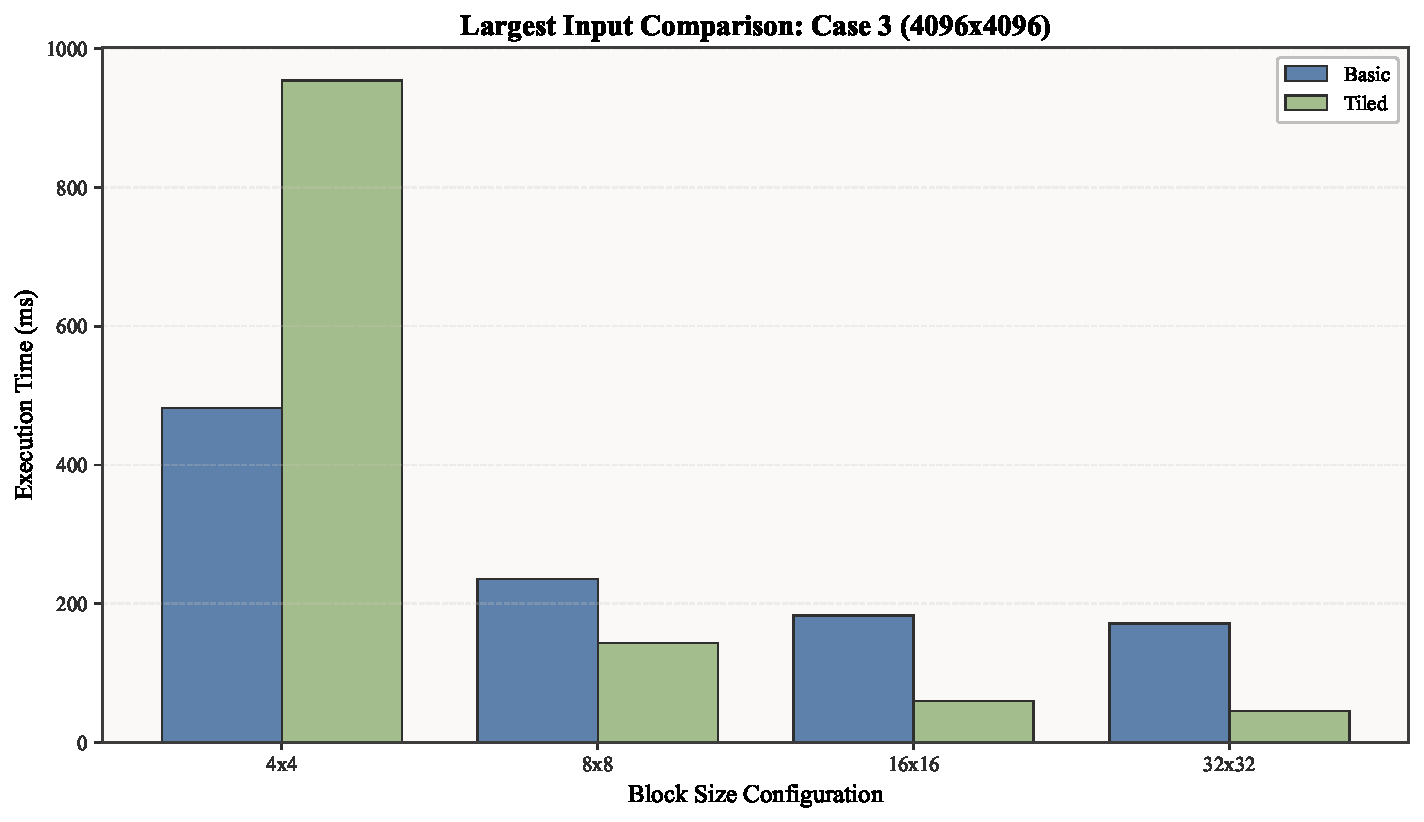
\includegraphics[width=0.9\textwidth]{../../ece569/build_dir/perf_analysis_graphs/plot3_largest_case_basic_vs_tiled.pdf}
	\caption{Basic matrix multiplication algorithm vs. tiled matrix multiplication algorithm on the largest plotted case.}
	\label{fig:comparison_plot}
\end{figure}


\section{Analysis \& Discussion}
This section answers the six required questions directly.
Each answer includes both the observed trend and a hardware-level root-cause explanation.

\subsection*{Question 1}
\textbf{Question:} Fix input size, discuss execution time trends with respect to change in thread block configuration for basic and tiled solutions individually. What is the optimal thread block configuration for each version? Discuss why a specific block size results with best/worst performance for each version. Does optimal block size depend on input size?\\
\textbf{Answer:} Fixix input size in Case 1,
 execution time falls as block size increases for both algorithms.
  The basic matrix multiplication algorithm drops
   from 120.1 ms at 4x4 to 43.2 ms at 32x32.
    The tiled matrix multiplication algorithm drops from
     251.0 ms at 4x4 to 11.1 ms at 32x32. The worst
      configuration is 4x4 and the best is 32x32 for
       this case. 
       The root cause is
        poor warp utilization at 4x4 and high synchronization
         overhead in the tiled matrix multiplication algorithm. The basic matrix multiplication algorithm is input dependent, since 16x16 outperforms 32x32 in Case 2 and Case 4. The tiled matrix multiplication algorithm remains best at 32x32 in the measured set.

\subsection*{Question 2}
\textbf{Question:} Discuss execution time trends among square matrices only for basic and tiled versions individually.\\
\textbf{Answer:} For square matrices, 
Case 1 and Case 2 have nearly the same arithmetic workload. 
Even so, runtime increases are much
 larger than the arithmetic increase. At 32x32, 
 the basic matrix multiplication algorithm rises 
 from 43.2 ms to 56.1 ms, a 29.9\% increase.
  The tiled matrix multiplication algorithm rises from 11.1 
  ms to 12.1 ms, a 9.0\% increase.
   This behavior indicates memory and boundary effects,
    not pure compute scaling.
     The root cause is divergence and boundary 
     inefficiency when dimensions are not clean multiples
      of the block size.

\subsection*{Question 3}
\textbf{Question:} Discuss execution time trends among square and non-square matrices for basic and tiled versions individually.\\
\textbf{Answer:} Both algorithms slow down as problem size
 grows from the smaller cases to the larger cases.
  The key difference appears in shape sensitivity.
   At 32x32, the basic matrix multiplication algorithm 
   increases from 171.3 ms in Case 3 to 214.5 ms in Case 4,
    which is a 25.2\% increase. The tiled matrix 
    multiplication algorithm stays essentially 
    flat at about 45.8 ms. The root cause is
     that irregular dimensions create boundary 
     blocks with partially inactive threads.
      The tiled matrix multiplication algorithm
       absorbs this cost better through shared-memory reuse.

\subsection*{Question 4}
\textbf{Question:} Discuss performance of basic and tiled solution versions for a given problem size and across different problem sizes. Include any additional plot that will help your claims.\\
\textbf{Answer:} For a fixed problem size in Case 3, the basic matrix multiplication algorithm is faster only at 4x4. The tiled matrix multiplication algorithm is faster at 8x8, 16x16, and 32x32, with speedups of 1.64x, 3.09x, and 3.74x. Across all tested sizes, this ranking is consistent. Appendix Figure \ref{fig:appendix_basic_combined} and Appendix Figure \ref{fig:appendix_tiled_combined} confirm the same trend over a wider workload range. The root cause is memory reuse. Shared-memory tiling reduces global memory transactions per output element and relieves bandwidth pressure.

\subsection*{Question 5}
\textbf{Question:} Can basic version execute faster than the tiled version for the same problem size? You need to use dataset\_generator to change the problem size and show execution time performance.\\
\textbf{Answer:} Yes. In the measured results,
 the basic matrix multiplication algorithm is faster 
 than the tiled matrix multiplication algorithm at 4x4
  for all tested problem sizes. In Case 1,
   the values are 120.1 ms and 251.0 ms.

\subsection*{Question 6}
\textbf{Question:} Can basic version run faster than the tiled version for the same block size? Your discussion needs to be based on your experimental results.\\
\textbf{Answer:} Yes. At block size 4x4, the basic matrix multiplication algorithm is faster than the tiled matrix multiplication algorithm in all four cases. At 8x8, 16x16, and 32x32, the tiled matrix multiplication algorithm is consistently faster. The root cause is a synchronization-heavy execution path in the tiled matrix multiplication algorithm at 4x4. At larger blocks, shared-memory reuse dominates and the tiled matrix multiplication algorithm wins. The crossover occurs between 4x4 and 8x8.

\section{Conclusion}
The measured data supports three direct conclusions.
First, 4x4 is consistently a poor configuration, especially for the tiled matrix multiplication algorithm.
Second, the tiled matrix multiplication algorithm provides strong speedups at practical block sizes, reaching 3.74x in this dataset.
Third, the tiled matrix multiplication algorithm is more robust to irregular dimensions than the basic matrix multiplication algorithm at larger scales.
These results highlight a central principle of GPU programming:
maximizing data reuse and memory locality often provides larger
performance gains than simply increasing raw computational throughput.
In practice, this study shows that carefully chosen block sizes
and shared-memory tiling are essential for achieving high
performance on modern GPU architectures such as the NVIDIA Tesla P100.

\appendix
\section{Appendix: Combined Scaling Plots}
These appendix figures combine first-run cases and performance-analysis cases in a single log-log view to extend the visible workload range.
They are intended to support the same conclusions, not replace the main analysis.

\begin{figure}[H]
	\centering
	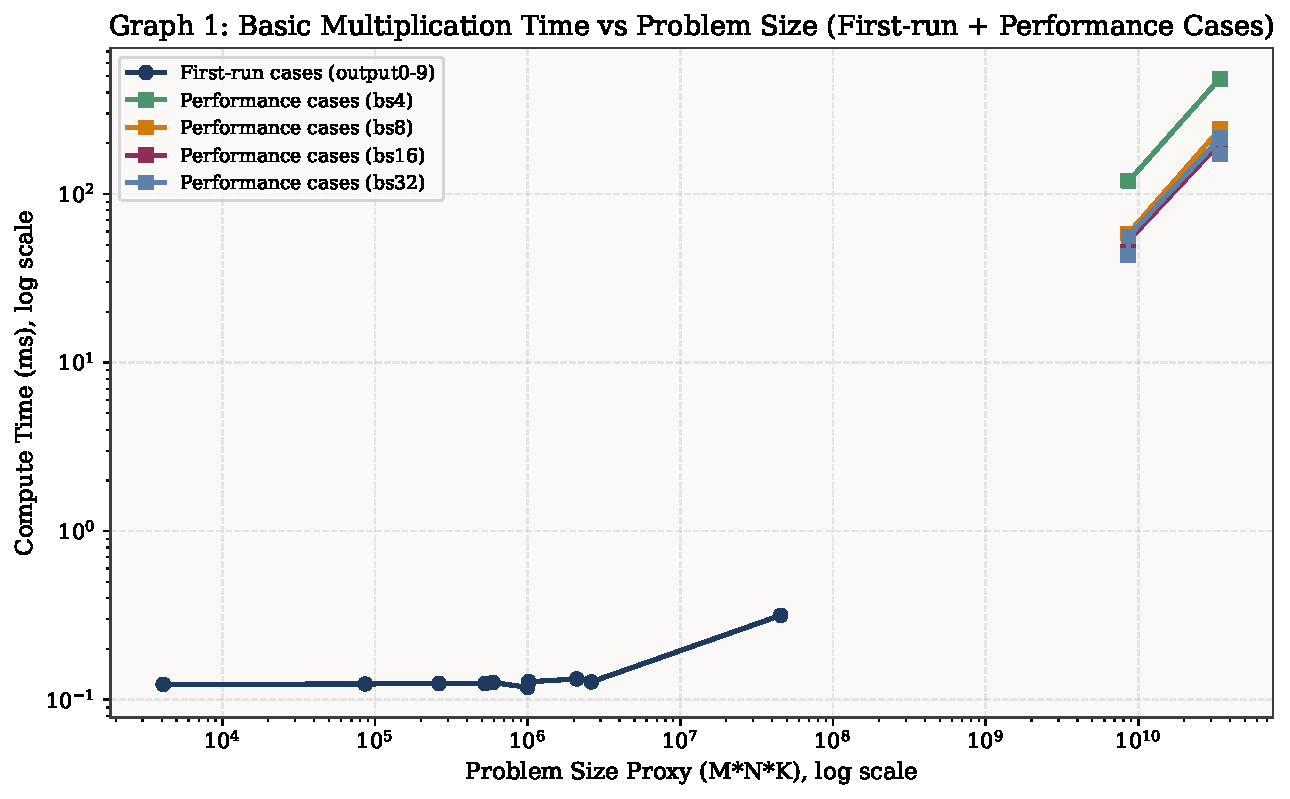
\includegraphics[width=0.95\textwidth]{../../ece569/build_dir/perf_analysis_graphs/graph1_basic_times_vs_size_combined.pdf}
	\caption{Appendix Graph A1: Basic multiplication time vs problem size (first-run + performance-analysis cases).}
	\label{fig:appendix_basic_combined}
\end{figure}

\begin{figure}[H]
	\centering
	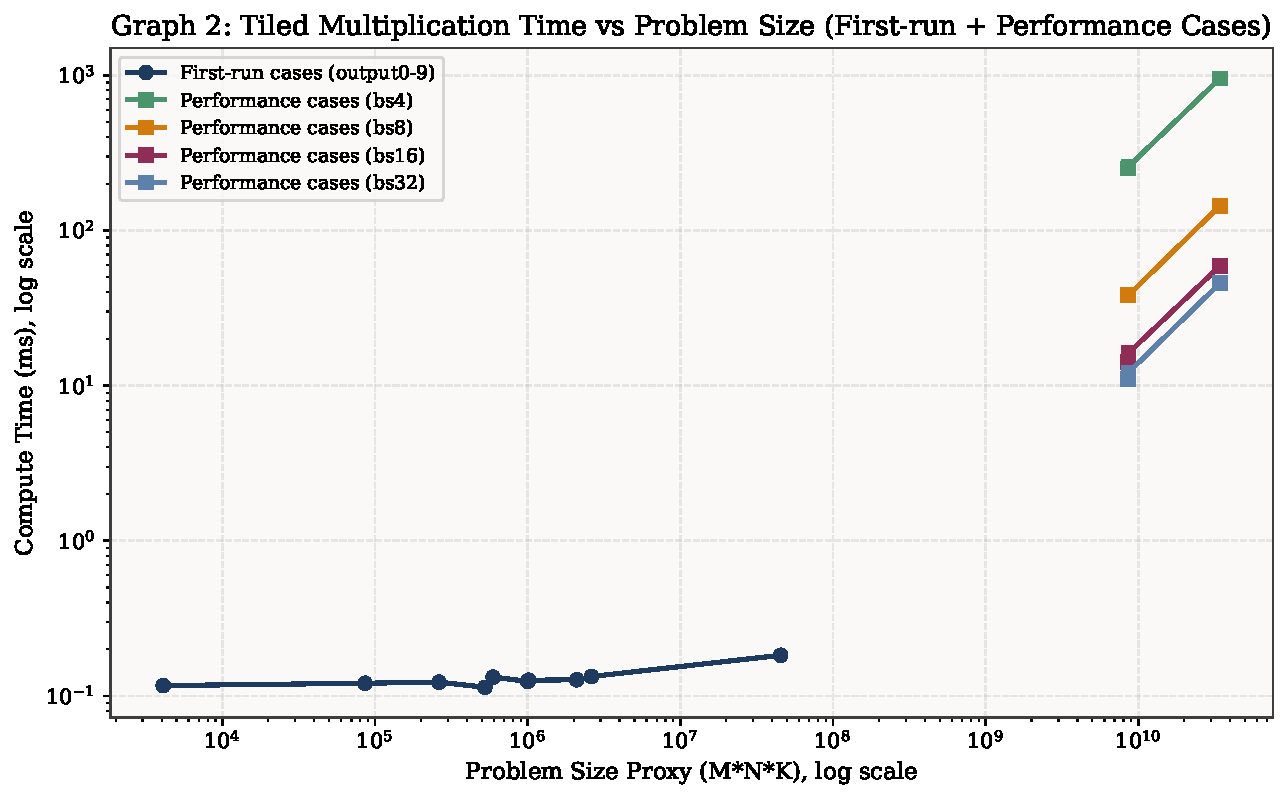
\includegraphics[width=0.95\textwidth]{../../ece569/build_dir/perf_analysis_graphs/graph2_tiled_times_vs_size_combined.pdf}
	\caption{Appendix Graph A2: Tiled multiplication time vs problem size (first-run + performance-analysis cases).}
	\label{fig:appendix_tiled_combined}
\end{figure}

\end{document}
